% Algorithms ~ A. Labouseur, Assignment 4 - Connor Fleischman

\documentclass[12pt, letterpaper]{article}
\usepackage{graphicx} % Required for inserting images
\usepackage{listings} % Required for inserting code
\usepackage{xcolor} % Required for formatting code
\usepackage{fancyhdr} % For custom headers and footers
\usepackage{titlesec} % For enhanced section titles
\usepackage{mathpazo} % For elegant fonts
\usepackage{tocloft} % For custom table of contents
\usepackage{appendix} % For appendices
\usepackage{hyperref} % For clickable links in TOC
\usepackage{amsmath, amssymb}
\usepackage{geometry}
\usepackage{bookmark}

\graphicspath{{./report/figures/}}
\lstset{language=C++, inputpath=./src/}
\geometry{a4paper, margin=1in}

% Custom Colors
\definecolor{background}{rgb}{0.84,0.84,0.84}
\definecolor{codegreen}{rgb}{0.2,0.7,0.2}
\definecolor{codeblue}{rgb}{0,0,0.7}
\definecolor{codegray}{rgb}{0.5,0.5,0.5}
\definecolor{codepurple}{rgb}{0.58,0,0.82}
\definecolor{codered}{rgb}{0.6,0,0}
\definecolor{keywordcolor}{rgb}{0.6,0,0.6}

% Custom Header and Footer
\pagestyle{fancy}
\fancyhf{}
\fancyhead[L]{\textit{Connor Fleischman - Assignment 4}}
\fancyhead[R]{\textit{Algorithms | Dr. Labouseur}}
\fancyfoot[C]{\thepage}
\setlength{\headheight}{14.5pt}


% Section Title Customization
\titleformat{\section}[block]{\Large\bfseries\color{black}}{\thesection}{1em}{}

% TOC (Link) Customization
\renewcommand{\cftsecfont}{\bfseries}
\renewcommand{\cftsecpagefont}{\bfseries}

% Define and set my code style
\lstdefinestyle{mystyle}{
   backgroundcolor=\color{white},   
   commentstyle=\color{blue},
   keywordstyle=\color{purple}\bfseries,
   numberstyle=\tiny\color{black},
   stringstyle=\color{gray},
   basicstyle=\ttfamily\tiny,
   frame=single, 
   rulecolor=\color{black},
   breakatwhitespace=false,         
   breaklines=true,                 
   captionpos=b,                    
   keepspaces=true,                 
   numbers=left,                    
   numbersep=10pt, 
   showspaces=false,                
   showstringspaces=false,
   showtabs=false,                  
   tabsize=4,
   emph={int,char,double,float,unsigned}, 
   emphstyle={\color{blue}},
}

\lstset{style=mystyle}

% Document Title and Metadata
\title{Assignment 4 - LaTeX Write-Up}
\author{Connor Fleischman}
\date{December 6, 2024}

% \begin{document}
\begin{document}

% Title Page
\pagenumbering{roman} % Start page numbering in i, ii..
\maketitle
\begin{center}
   
\includegraphics[width=120mm,scale=0.5]{MaristSeal.png}
\end{center}
\newpage

% Table of Contents
\tableofcontents
\newpage
\setcounter{page}{1} % Start page numbering at 1
\pagenumbering{arabic} % Start page numbering in 1, 2..

\section{Introduction}
\textbf{Assignment 4} requires implementing a Directed Graph (\ref{Graph}) and some Spices and Knapsacks (\ref{SpiceKnapsack}) and running algorithms on them.
To do this I modified the Undirected Graph class from \textbf{Assignment 3} to include weighted edges between the vertices.
Then, with each graph described in \texttt{graphs2.txt} (\ref{Graph_ParseBuild}) , beginning with the first vertex in the graph, a Single Source Shortest Path algorithm is performed (\ref{Graph_SSSP}) .
Next, after building the spices and knapsacks described in \texttt{spice.txt} (\ref{SpiceKnapsack_ParseBuild}) , each knapsack is filled using the Fractional Knapsack algorithm (\ref{SpiceKnapsack_FKA}).
Finally, all graphs, spices, and knapsacks are destroyed and their memory freed (\ref{CleanUp}).

\section{Directed Graphing} \label{Graph}
To implement a Directed Graph and perform a Single Source Shortest Path (SSSP) algorithm on the first vertex, one must:
\begin{itemize}
   \item Read and parse the data in \texttt{graph2.txt}
   \item Build each graph described in the file
   \item Perform a SSSP algorithm on the first vertex to all other connected vertices
   \item Destroy the graph and allocate memory
\end{itemize}

\subsection{Parsing \& Building} \label{Graph_ParseBuild}
The \texttt{graph2.txt} file is formatted in such a way so that each line contains one instruction.
Each graph begins with the 'new' command followed by some number of 'new vertex' or 'new edge' commands.
Lines beginning with '-', the comment symbol, are dropped.
\begin{center}
   \lstinputlisting[language=C++, caption=Parsing Implementation, firstline=11, lastline=52]{Parse.h}
\end{center}
My implementation opens and reads the file.
Then every line in the file is read and parsed.
Comments are skipped and all other lines are pushed back to the returned graphs vector of vectors.
Every 'new graph' command starts a new graph vector which, when finished being parsed, will be pushed back into the larger vector.
\vspace*{5px}
\newline
Once parsing is complete this vector of vectors of strings, graphs, is built.
In the main file, each individual graph in graphs is put through the build function.
Build takes every instruction in a graph and builds that graph with some specified number of vertices and edges (with their own weights).
\begin{center}
   \lstinputlisting[language=C++, caption=Building Implementation, firstline=16, lastline=57]{Build.h}
\end{center}
Firstly, a flag to track the first vertex in the graph and a placeholder for the first vertex's ID are created.
Then every instruction in the provided graph is read and interpreted.
The instruction is broken into individual words.
Next, depending on the first word, an edge or vertex is built for that graph.
After all instructions are interpreted, the first vertex's ID is returned.
\begin{center}
   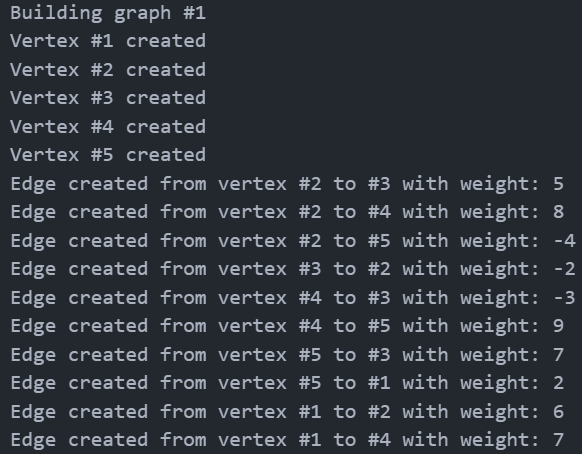
\includegraphics{images/Graph1_ParseBuild.png}
\end{center}
Here we see that, for \textbf{Graph 1}, five vertices are created and ten edges are created between the vertices.
Each characterized by some weight.

\subsection{Single Source Shortest Path Algorithm} \label{Graph_SSSP}
After the graph is built, using the first vertex returned by the build function, a Single Source Shortest Path algorithm is ran.
This algorithm calculates the path of least cost from some source to every available sink.
It does this by performing every possible traversal from the source to every possible sink.
While doing this it keeps track of the most efficient, lest costly, path.
Once all pathways are traversed, and the best routes calculated, the program displays these shortest paths.
\begin{center}
   \lstinputlisting[language=C++, caption=SSSP Implementation, firstline=221, lastline=268]{graph/DirectedGraph.h}
\end{center}
In the above code we see that mapPathways takes in some starting vertex ID and searches for the vertex.
Once found, its distance is set to 0, since it's the source.
Then for every other vertex, the path from the source to that vertex is calculated.
If that path is shorter than the existing path to that vertex, it is updated.
Then once all vertices have been mapped a check is ran to see if all shortest paths were mapped.
Finally the result is output along with the path taken to get from the source to that sink.
\vspace*{5px}
\newline
The below function is a helper-function for outputting the shortest path:
\begin{center}
   \lstinputlisting[language=C++, caption=SSSP Helper, firstline=48, lastline=57]{graph/DirectedGraph.h}
\end{center}
This uses recursion to take the path of the most efficient route from sink to source and reorder it in reverse to get the correct path displayed.
Resulting in a path from source to sink, instead of backwards.

\section{Spices \& Knapsacks} \label{SpiceKnapsack}
The remaining workload of \textbf{Assignment 4} consists of creating certain spices and knapsacks.
Each spice is characteristics by a color, some total price, and a quantity.
The unit price for a spice is also calculated.
A knapsack is characterized simply as some number, describing the capacity of the knapsack.
\vspace*{5px}
\newline
To fulfill this we must:
\begin{itemize}
   \item Read and parse the spices and knapsacks in \texttt{spices.txt}
   \item Build all spices with their respective characteristics
   \item Build all knapsacks with their respective capacities
   \item Perform a fractional knapsack algorithm for each knapsack on all spices
   \item Destroy all knapsacks and spices and allocate memory
\end{itemize}

\subsection{Parsing \& Building} \label{SpiceKnapsack_ParseBuild}
The input file \texttt{spices.txt}, being so similarly formatted to \texttt{graph2.txt}, requires some of the same logic as before too.
However, unlike before, \texttt{spices.txt} does not have one instruction per line.
Instead, the line containing the spice characteristics contains multiple instruction, one per characteristic.
This results in an increase in complexity as when parsing a spice, we must parse each instruction on the line, instead of just the whole line.
\vspace*{5px}
\newline
To achieve this, I broke my logic into two main sections, parsing the whole of \texttt{spice.txt}, and parsing a specific line into its individual instructions.
This allows for reduced complexity and an easier overall time understanding the code.
\begin{center}
   \lstinputlisting[language=C++, caption=Parsing File Implementation, firstline=55, lastline=78]{Parse.h}
\end{center}
TODO:
\begin{center}
   \lstinputlisting[language=C++, caption=Parsing Instruction Implementation, firstline=80, lastline=114]{Parse.h}
\end{center}
TODO:
\begin{center}
   \lstinputlisting[language=C++, caption=Building Implementation, firstline=1, lastline=5]{Build.h}
\end{center}
TODO:
\begin{center}
   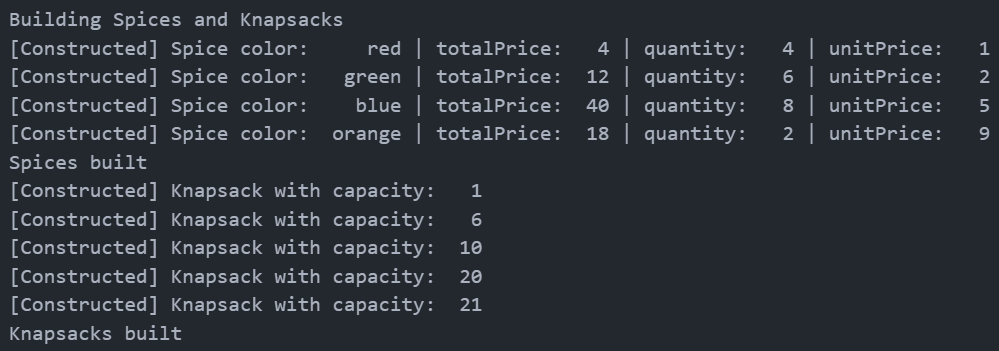
\includegraphics{images/SpiceKnapsack_ParseBuild.png}
\end{center}

\subsection{Fractional Knapsack Algorithm} \label{SpiceKnapsack_FKA}
TODO:

\section{Clean Up} \label{CleanUp}
\begin{center}
   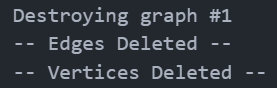
\includegraphics{images/Graph1_CleanUp.png}
\end{center}
TODO:
\begin{center}
   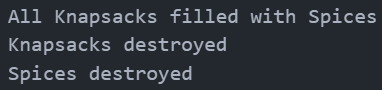
\includegraphics{images/SpiceKnapsack_CleanUp.png}
\end{center}
TODO:

\section{Miscellaneous Implementations} \label{MiscImp}
TODO:

\end{document}
